
\chapter{Inequalities in Mean Age at First Hospital Admission}

%----------------------------------------------------------------%%----------------------------------------------------------------%

\vspace{0.5in}

\textbf{Paper:}
\textsc{Rosie Seaman, \underline{Andreas H\"ohn}, Rune Lindahl Jacobsen, 
	    Pekka Martikainen, Alyson van Raalte, and Kaare Christensen:} 
		Rethinking Morbidity Compression: Increasing Inequality in Age 
		at Morbidity Onset. \textbf{\textit{Submitted to a peer-reviewed journal}}		


%----------------------------------------------------------------%%----------------------------------------------------------------%


%%% ABSTRACT %%%

\newpage

\section{Abstract}
% BACKGROUND %
\textbf{Background:} To evaluate morbidity compression, studies typically 
report the proportion of life expectancy spent in an unhealthy state. This 
overlooks variation in age at morbidity onset between individuals, a factor 
Fries (1980) saw as crucial for determining whether the continuation of 
disease postponement was possible. We use incidence of first hospitalization 
after age 60 to study variation in morbidity onset over a 27-year period 
in Denmark. \newline
% METHODS %
\textbf{Methods:} Number of hospitalizations and the population at risk 
for each year between 1987 and 2014 were identified using nationwide 
registry data. Sex-specific life tables were constructed, from which 
the mean and the coefficient of variation in age at first admission were 
calculated. \newline
% RESULTS %
\textbf{Results:} Mean age at first admission increased between 1987 
and 2014 from 67.8 years (95\% CI: 67.7 - 67.9) to 69.5 years (95\% CI: 
69.4 - 69.6) in men, and 69.1 (95\% CI: 69.1 - 69.2) to 70.5 years (95\% 
CI: 70.4 - 70.6) in women. In the same period, the coefficient of variation 
in age at first admission increased from 9.1\% (95\% CI: 9.0 - 9.1) to 
9.9\% (95\% CI: 9.8 - 10.0) among men and from 10.3\% (95\% CI: 10.2 - 
10.4) to 10.6\% (95\% CI: 10.5 - 10.6) among women. \newline
% CONCLUSION %
\textbf{Conclusion:} On average, morbidity has been postponed but variation 
in age at onset has increased. This variation has important implications for 
individual life planning and population-level welfare. Pensions, social and 
healthcare services will have to adapt to an increasingly heterogeneous aging 
population, a phenomenon that trends in the measurement of average morbidity 
onset cannot identify. 


\newpage


%----------------------------------------------------------------%%----------------------------------------------------------------%


\section{Key Messages}

\begin{enumerate}
	\item	Morbidity compression means that years of bad health should become 
			increasingly concentrated at the end of life. Typically, compression 
			is measured in terms of changes in the proportion of average time 
			spent in an unhealthy state. This approach assumes that the same 
			average gain has been achieved for everyone, or that differences 
			between individuals have stayed constant over time.
	\item	Inequality in morbidity onset across all individuals has largely 
			been overlooked. Part of the problem is the challenge associated 
			with estimating morbidity incidence.
	\item	Hospital admissions, among older ages, have been used to measure 
			the onset of individual-level health deterioration. Routinely 
			collected hospital admission data allow estimates of incidence 
			of overall morbidity at the population level, from which variation 
			in age at onset can be calculated.
	\item	We show that, on average, morbidity has been postponed towards 
			older ages. Alongside this, variation between individuals has 
			increased, suggesting that population health is becoming more 
			heterogeneous. 
	\item	Monitoring variation in age at morbidity onset is important for 
			planning pensions, social care, and health services which will 
			have to adapt to the heterogeneous needs of aging populations, 
			something that average morbidity measures cannot identify.
\end{enumerate}


\newpage


%----------------------------------------------------------------%%----------------------------------------------------------------%


\section{Background}

Remaining life expectancy at age 60 has rapidly increased across developed 
countries.\citep{mathers2015causes} Whether the extra years of life are spent 
in good or bad health remains unclear, and depends in part on how health is 
measured.\citep{christensen2008exceptional,christensen2009ageing,parker2007health,
beltran2015past,beltran2014going,fries2011compression} Fries (1980) proposed 
a scenario where 'the amount of disability can decrease as morbidity is compressed 
into the shorter span between the increasing age at onset of disability and 
death'.\citep{fries1980aging} Gruenberg (1977) was more pessimistic, arguing 
that technological advancement would allow people to live for longer but in 
a prolonged state of poor health.\citep{gruenberg1977failures} Manton (1982) 
suggested that falling mortality rates would be associated with a change in 
the distribution of disease types.\citep{manton1982changing} Specifically, 
an increase in the proportion of years spent with moderate health conditions 
and a decrease in the proportion of years spent with serious health conditions. 
Monitoring the rate of change in disability-free life expectancy (DFLE) or 
healthy life expectancy (HLE), compared with the rate of change in mortality, 
is assumed to be the best way to evaluate which scenario might be emerging 
as populations are aging.\citep{robine1991healthy,robine1998examination,
sanders1964measuring,sullivan1971single}  If gains in DFLE or HLE are greater 
than gains in average life expectancy, morbidity compression is likely. If 
gains in average life expectancy are greater, it would be considered as evidence 
of expansion.

Key to Fries (1980) theory of morbidity compression is that alongside increasing 
age at death, the years spent with bad health or disability would become 
increasingly concentrated at the end of life. This implies that population 
age distributions of morbidity would become increasingly homogeneous among 
individuals. However, this important piece of information for determining 
whether the continuation of disease postponement is possible, has been 
overlooked in the morbidity compression debate.\citep{stallard2016compression}
Therefore, it is not known whether improving average health has been accompanied 
by decreasing or increasing variation in the age of morbidity onset between 
all individuals. Changes in the age distribution of morbidity onset have 
individual-level and population-level implications beyond theory. For individuals, 
it represents the amount of uncertainty in the timing of health deterioration. 
At the macro-level, pensions, social care, and health services will have to 
adapt to the heterogeneous needs of ageing populations, something that average 
measures cannot identify.\citep{van2018case}

To estimate the age distribution of morbidity onset across all individuals, 
we need to distinguish between incidence and prevalence.\citep{fries2011compression} 
Estimating incidence is challenging from cross-sectional health 
surveys.\citep{robine1991healthy} Administrative healthcare data provide 
an opportunity and are continuously updated. Number of hospital days, number 
of admissions, and cause of admission have been operationalized to capture 
health.\citep{busse2002use,dixon2004hospital,oksuzyan2013changes,simmonds2014understanding,
hu2018changes,hohn2018sex,luben2016predicting,syddall2016understanding} 
In this paper, we quantify changes in the age distribution of morbidity 
onset across all individuals aged 60+ between 1987 and 2014, using first 
hospital admission for all causes among Danish men and women. Denmark is 
a valuable case study country because the aging population structure is 
comparable to many other developed countries. Unique to Denmark is that 
data exist for constructing individual-level hospitalization trajectories 
for the total population covering a substantial period of time.\citep{schmidt2015danish,
westergaard2019population} \\


%----------------------------------------------------------------%
%----------------------------------------------------------------%


\section{Methods and Materials}

\subsection{Data Sources}

We used individual-level register data covering the total Danish population 
aged 60+. We linked records from the National Patient Register (NPR) with 
data from the Central Population Register (CPR) using the unique personal 
identification number (CPR-Number). The NPR, a population-based register, 
contains information on all treatments provided in Danish hospitals since 
1977. Reporting of hospital admissions is compulsory, leading to high levels 
of completeness and reliability. The CPR includes socio-demographic information 
on the population alive and residing in Denmark since 1968, including sex, 
place and date of birth, and date of death.\citep{schmidt2015danish,schmidt2014}\\

\subsection{Study Population}

In an ideal scenario, we would have health information for all individuals, 
covering the entire life course. This would have allowed us to identify every 
entry into, and every recovery from, an unhealthy state. As hospitalization 
data for Denmark began in 1977, we cannot identify admissions before this year. 
Therefore, we created an identical cohort study population for each calendar 
year by consistently applying the same method for each year between 1987 
(to allow for a washout period) and 2014. This approach means that all estimated 
values were comparable throughout the study period. \hyperref[ch4:fig1]{Figure 1} summarizes the 
process of identifying the study population in 1987 as an example year.\\

	%------------------%
	\begin{figure}[H]
		\centering
		\includegraphics[scale=0.60]{Paper_3/Figure_1.pdf}
		\caption*{\textbf{Figure 1:} 	Constructing the Cohort Study Population: 
										Example Year 1987.}
	\label{ch4:fig1}
	\end{figure}
	%--------------------%


First, we linked CPR and NPR information on all inpatient admissions and the 
population alive and residing in Denmark aged 60+. Second, we identified all 
individuals hospitalized within the previous 7-year period -- irrespective 
of length of stay, and excluded these individuals from the analyses for the 
particular year. Guided by existing literature,\citep{modig2017estimating,
roberts2015revisiting} a 7-year washout period was used to limit the chance 
that a first event was a readmission or a follow-up treatment. Third, for the 
remaining Danes, we identified the population at risk and the first events 
within each calendar year. We defined first events as the first inpatient 
hospitalization after age 60, from all causes, lasting for at least two days.
We included all fatal events regardless of length of admission. This definition 
is likely to capture hospital admissions that would require inpatient care 
consistently throughout the study period.  Events were included regardless 
of whether the outcome was death or discharge. Trends over time in the number 
of individuals at risk, first events, and those excluded in the washout period 
are given in \hyperref[ch4:app1]{Appendix 1}. \\

\subsection{Statistical Analysis}

From the number of first hospital admissions and the population at risk, we 
estimated the age-specific risks of first admission ($q_{x,t}hosp$), for each 
age $x$ and each calendar year $t$. Age-specific risks of first admission were 
calculated for men and women separately. We constructed life tables for each calendar 
year using standard demographic methodology.\citep{preston2000demography} 
Using the age-specific risks to have a first event at age $x$ in year $t$ ($q_{x,t}hosp$), 
we estimated $e_{x,t}hosp$, which is conditional upon survival to age 60. The 
definition of $e_{x,t}hosp$ is equivalent to the definition of remaining life 
expectancy at age $x$ in year $t$ ($e_{x,t}$) in a period life table. It quantifies 
the remaining average number of years until the event takes place for an 
individual of exact age $x$, given hospitalization patterns of year $t$.  In 
our case, $e_{x,t}hosp$ quantified the expected average number of years until 
the first hospital admission for a person who is aged $x$ in year $t$. Adding 
$60$ to the value of $e_{x,t}hosp$ allowed the interpretation to be mean age at 
first hospital admission lasting for a minimum of 2 days, including cases 
that ended in death or discharge.

We measured between individual variation in age at first hospital admission 
using the coefficient of variation (CoefV) and reported values as a percentage. 
The CoefV is a standard measure of dispersion and is defined as the ratio 
of the standard deviation to the mean. Here, the CoefV reflects the variability 
in age at first hospital admission relative to the mean age at first hospital 
admission. We calculated 95\% Confidence Intervals (95\% CIs) for $e_{x,t}hosp$ and 
CoefV.\citep{chiang1984lifetable}\\


%----------------------------------------------------------------%
%----------------------------------------------------------------%


\section{Results}

\subsection{Trends in Mean Age}

	%------------------%
	\begin{figure}[H]
		\centering
		\includegraphics[scale=0.475]{Paper_3/Figure_2.pdf}
		\caption*{\textbf{Figure 2:} 	Trends in Mean Age at First Hospital 
										Admission for Men and Women Age 60, 1987 to 2014.}
	\label{ch4:fig2}
	\end{figure}
	%--------------------%

\hyperref[ch4:fig2]{Figure 2} shows trends in mean age at first admission. 
The trend demonstrates a subtle u-shaped pattern between 1987 and 2014. The trend declined in the 
1990s before rebounding in the 2000s. In 1987, the mean age at first admission 
for men was 67.8 years (95\% CI: 67.7 - 67.9). At the midpoint, 2001, mean 
age had increased onlz slightly to 67.9 years (95\% CI: 67.8 - 67.9). By 2014, 
mean age at first admission had increased to 69.5 years (95\% CI: 69.4 - 
69.6). For women, the mean age decreased slightly between 1987 and 2001: 
from 69.1 years (95\% CI: 69.1 - 69.2) to 68.5 years (95\% CI: 68.4 - 
68.6). By 2014, mean age for women had increased to 70.5 years (95\% CI: 
70.4 - 70.6).\\

\subsection{Changes to the Age Distribution}

\hyperref[ch4:fig3]{Figure 3} shows the age distribution of first hospital 
admission in 1987, 2001 and 2014.

	%------------------%
	\begin{figure}[H]
		\centering
		\includegraphics[scale=0.475]{Paper_3/Figure_3.pdf}
		\caption*{\textbf{Figure 3:} 	Distribution of Age at First Hospital 
										Admission Across ages 60+ in 1987, 2001 and 2014.}
	\label{ch4:fig3}
	\end{figure}
	%--------------------%

We focus on the change in the distribution of first events 
from the age groups 60-69 to age 70+, the age groups surrounding the mean 
age at first admission. In 1987, 69.6\% of all men experienced their first 
admission to hospital between age 60 and 69, while 30.4\% of all men had 
their first admission at ages 70+. By 2001, the proportion among men aged 
60 to 69 remained similar at 69.0\%, before decreasing to 58.8\% in 2014. 
Among women, the proportion who experienced a first admission at age 60-69 
was 61.8\% in 1987, while 38.1\% experienced a first admission at ages 70+. 
In contrast to men, the proportion of women aged 60-69 who experienced a 
first admission in 2001 increased to 65.1\%. By 2014, 53.3\% of women aged 
60 to 69 experienced a first admission and 46.7\% experienced a first admission 
at ages 70+.\\

\subsection{Trends in the Coefficient of Variation}

To quantify changes in the age distribution, we estimated the CoefV. As shown 
in \hyperref[ch4:fig4]{Figure 4}, we found a u-shaped pattern. Among men, the CoefV in average age 
at first admission at age 60 decreased from 9.1\% (95\% CI: 9.0 - 9.1) in 1987 
to 8.7\% (95\% CI: 8.6 - 8.7) in 2001. For women, the corresponding change was 
from 10.3\% (95\% CI: 10.2 - 10.4)  to 9.4\% (95\% CI: 9.4 - 9.5). In the early 
2000s, the trends in variation changed to increasing. In 2014, the CoefV was 
9.9\% (95\% CI: 9.8 - 10.0) for men and 10.6\% (95\% CI: 10.5 - 10.6) for women.\\

	%------------------%
	\begin{figure}[H]
		\centering
		\includegraphics[scale=0.475]{Paper_3/Figure_4.pdf}
		\caption*{\textbf{Figure 4:} 	Trends in the CoefV in Mean Age at First 
										Hospital Admission (\%) for Men and Women 
										Age 60, 1987 to 2014.}
	\label{ch4:fig4}
	\end{figure}
	%--------------------%

\subsection{Sensitivity Analyses}

Our main results reflect hospital stays lasting a minimum of 2 days, including 
all fatal events. The direction of the trends were consistent in three sensitivity 
tests. First, we varied the minimum length of stay from 2 days to 1 day, 3 days, 
5 days, and 7 days. Second, we excluded fatal cases that occurred between the 1st 
day of admission and the minimum length of stay. Third, we changed the washout 
period length from 7 years to 5 years, and 10 years. Results for sensitivity 
checks and further details are given in \hyperref[ch4:app2]{Appendix 2} and 
\hyperref[ch4:app3]{Appendix 3}.\\


%----------------------------------------------------------------%
%----------------------------------------------------------------%


\section{Discussion}

\subsection{Summary of Findings}

Average age at first admission at age 60 was higher in 2014 than in 1987. 
The number of first admissions at ages 60-69 reduced during this period. These 
findings indicate that people became healthier across these ages. However, 
the shifting of events towards older ages meant that the age distribution of 
first hospital admission widened over time, causing the coefficient of variation 
to increase. In pragmatic terms, higher variation in age at first hospital 
admission after age 60 translates into greater uncertainty for individuals 
in the timing of the onset of morbidity. At the macro-level, it indicates 
that population health is becoming increasingly heterogeneous.\\


\subsection{Interpretations and Implications}

Many people are aging with better health today than in the past. Healthy aging 
is due to multiple life course factors, including improved health during childhood, 
reduced exposure to hazardous working conditions, and changes in health behaviors 
such as smoking or diet.\citep{vaupel2010biodemography,brandt2012tracing} 
Another contributing factor is that technological advancement has enabled 
more individuals to survive longer in better health. Although some chronic 
diseases may show increased prevalence over time (e.g. diabetes) they may 
now lead to a hospital admission later in life. Perhaps the strongest example 
of this, is the treatment of hypertension and cardiovascular diseases.\citep{blacher2016epidemiological} 
Treatment has changed dramatically over time and mortality has declined, leading 
to more people surviving without serious cardiovascular events and only being 
admitted to hospital later in life. This observation is consistent with our 
results showing the redistribution of first events from younger to older ages.

At the same time, our results show increasing diversity in healthy aging. The 
same technological advancements that have postponed major health events, have 
also enabled individuals to live for longer while managing chronic 
conditions.\citep{gruenberg1977failures,reeves2018challenge,engelman2010implications} 
Greater variation between individuals in age at first hospital admission 
could therefore be due to more heterogeneous health profiles arising from 
an increased prevalence of chronic conditions. Additionally, some components 
of increasing health variation could have their roots in the changing epidemiological 
environment experienced by older adults as infants and children. As infectious 
diseases became increasingly controlled, weaker individuals that would have 
died as children in previous decades survived to older ages, making for a more 
heterogeneous population at older ages.\citep{engelman2010implications} Our 
results for morbidity echo findings for mortality which have shown that increased 
survivorship has been accompanied by increasing population-level heterogeneity 
in age at death at these older ages.\citep{stallard2016compression,engelman2010implications}\\

\subsection{Methodological Considerations}

Linked hospital admission data have been used to investigate health at older 
ages and across multiple countries.\citep{busse2002use,dixon2004hospital,
oksuzyan2013changes} Studies clearly demonstrated that these data can be 
used to derive powerful indicators of health. A particular strength of our 
study is that we were able to identify individual patient trajectories to 
derive incidence-based estimates.\citep{fries2011compression,westergaard2019population} 
We used the most accurate population denominators for those at risk of admission. 
Other countries may only be able to identify prevalence-based measures, based 
on the number of admissions and using an inaccurate total population denominator. 
Our data allowed us to identify all events during the study period and determine 
the exact age at event for all individuals. Studies using survey data are often 
restricted to picking up events retrospectively and may miss out events. While 
standardized, self-reported measures are powerful, there are limitations in 
terms of recall bias, selectivity, and subjectivity.

We attempted to exclude re-admissions to hospital by applying a 7-year washout 
period at each calendar year. While a 7-year washout period will not fully remove 
all cases of readmission, it was a length of time that reflected established choices 
in the existing clinical research literature.\citep{modig2017estimating,roberts2015revisiting}

Accounting for the impact of population-level changes in admission strategies is 
challenging. To address this issue, we obtained an overview of admissions using 
19 causes of admission for the entire study period by utilizing harmonized ICD-8 
and ICD-10 codes (\hyperref[ch4:app4]{Appendix 4}). While the relative contribution from some causes 
decreased over the study period, other causes increased or remained stable. 
Studying a change in admission strategy requires consistent, detailed information 
on inpatient, outpatient, and primary healthcare attendances by cause of admission 
and length of treatment. In Denmark, outpatient data and primary healthcare data 
do not contain suitable information for carrying out such analyses.

A major aim of current healthcare strategies is to reduce length of stay. This 
is driven by the assumption that shorter stays are more cost effective. We investigated 
the potential impact of changing the minimum length of stay on our results by repeating 
all stages of the analyses for hospital stays lasting for at least 1 day, 3 days, 
5 days, and 7 days (\hyperref[ch4:app2]{Appendix 2}). We found a step-wise increase 
in the mean and the variation in the age at first admission with every increase in minimum length of 
stay, but no change in the trend direction. Patients in Denmark in 2015 stayed in 
hospital for an average of 5.5 days, which is one of the shortest average lengths 
of stay in hospital within Europe.\citep{oecd2017indicators} Our main results define 
an admission as lasting for a minimum of 2 days which is likely to capture conditions 
that would always require inpatient care over the entire study period and does not 
bias the trends that are documented.\\

\subsection{Concluding Theoretical Reflections}
Studies of morbidity compression have consistently calculated the average proportion 
of time spent in an unhealthy state, relative to average length of life.\citep{beltran2015past,
salomon2012healthy,crimmins2016trends,colvez1983potential,robine1999health,
murray2012disability} This only reflects part of Fries' theory of morbidity 
compression. To understand whether the continuation of disease postponement 
is possible 'analysis of variation, not of mean values, becomes crucial'.\citep{fries1980aging} 
Although, it has been forty years since Fries linked the measurement of the 
standard deviation between individuals to the concept of morbidity compression, 
empirical measurement of variation has been overlooked. In this study, we measure 
variation in the age of morbidity onset between all individuals, using first 
hospital admission at ages 60 and older. Measuring the age distribution of 
morbidity onset across all individuals underlines that the concept of morbidity 
compression is more nuanced than has previously been conceived. Incorporating a 
variation perspective into morbidity studies is important for individual life 
planning and population-level welfare. Pensions, social care and health services 
will have to adapt to the heterogeneous needs of aging populations, something 
that average morbidity measures cannot identify.\\


%----------------------------------------------------------------%
%----------------------------------------------------------------%


\newpage


\section{Supplementary Material}

\vspace{0.25in}


\subsection{Appendix 1}
	%------------------%
	\begin{figure}[H]
		\centering
		\includegraphics[scale=0.5]{Paper_3/Appendix_1.pdf}
		\caption*{\textbf{Figure Appendix 1:} 	Absolute number of individuals at 
												risk, first events, and individuals 
												excluded during the washout period 
												for each year in the study period.}
	\label{ch4:app1}
	\end{figure}
	%--------------------%


%----------------------------------------------------------------%
%----------------------------------------------------------------%


\newpage

\subsection{Appendix 2}

\label{ch4:app2}

The impact of changing the length of stay in hospital was tested by repeating all 
stages of the analysis for hospital stays lasting 1 day, 3 days, 5 days and 7 days. 
We found a stepwise increase in the mean age at first admission and variation with 
every increase in length of stay. The trends over time followed the same overall 
patterns, within the context of different absolute levels. Stays lasting 1 day were 
an exception as mean age at first admission and the variation were slightly decreasing 
over the entire study period. In 2007, changes in the administrative structuring of 
healthcare in Denmark resulted in temporary changes in the trends for 1 day. Results 
for stays lasting for 2 days or longer were not affected.

Removing deaths that occurred during an admission to hospital increased the mean age 
at first admission and increased variation slightly. This is evidence that removing 
deaths introduces a selection bias in our study population as individuals who died 
during an admission to hospital were admitted at slightly younger ages. There was 
no difference in the trends including and excluding fatal events for lengths of stay 
lasting only 1 day. Restricting the length of stay to 1 day means that cases could 
not go on to have a longer length of stay. This is equally true if an admission ended 
in fatality that occurred on the first day of admission.


\begin{landscape}

	%------------------%
	\begin{figure}[H]
		\centering
		\includegraphics[scale=0.65]{Paper_3/Appendix_2.pdf}
		\caption*{\textbf{Figure Appendix 2:} Trends in Mean Age and CoefV (in \%) of 
											First Hospital Admission for Men and Women, 
											1987 to 2014, for Varying Lengths of Hospital 
											Admission and Comparing the Impact of Fatal Events.}
	\end{figure}
	%--------------------%
	
\end{landscape}


%----------------------------------------------------------------%
%----------------------------------------------------------------%


\subsection{Appendix 3}

\label{ch4:app3}

Our main results used a 7-year washout period. We repeated all of our analyses 
for hospital admission lasting a minimum of 2 days using a 5-year washout period 
and a 10-year washout period for comparison. The mean age trends and CoefV trends 
comparing the different washout period lengths are shown in Appendix Figure 3. The first 
time point where the data are comparable for all three washout period lengths is 
1990. The  difference in the trends prior to 1990 are due to the fact that different 
background data is being used. The trends converge for all three wash-out period 
lengths over the study period. Therefore the impact of changing the length of 
wash-out period was minimal. \\

\begin{landscape}


	%------------------%
	\begin{figure}[H]
		\vspace{0.25in}
		\centering
		\includegraphics[scale=0.775]{Paper_3/Appendix_3.pdf}
		\caption*{\textbf{Figure Appendix 3:}	Trends in Mean Age at First Hospital 
											  	Admission and CoefV (in \%)for Men and Women Age 60, 1987 
												to 2014, Comparing Different Lengths of 
												Washout Period.}
	\end{figure}
	%--------------------%


\end{landscape}

%----------------------------------------------------------------%
%----------------------------------------------------------------%


\newpage

\subsection{Appendix 4}

	%------------------%
	\begin{figure}[H]
		\centering
		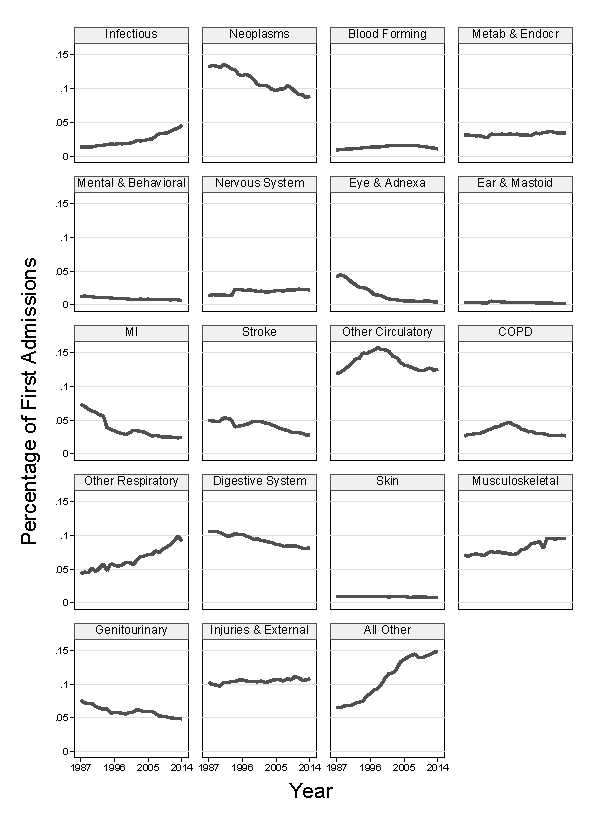
\includegraphics[scale=1.35]{Paper_3/Appendix_4.pdf}
		\caption*{\textbf{Figure Appendix 4:} 	Percentage of first hospital admission 
												at age 60+ by 19 cause specific groups 
												for yearly study population, 1987 to 
												2014. Cause specific categories constructed 
												from harmonized ICD-8 and ICD-10 codes 
												(Danish modification).}
	\label{ch4:app4}
	\end{figure}
	%--------------------%
	
	
%----------------------------------------------------------------%
%----------------------------------------------------------------%
